

% 
% chapter2.tex
% ThesisISEL
% 
% Created by Serge Lage on 2019/07/30.
%
% ================
% = State of the Art =
% ================
\chapter{State of the Art}
\label{cha:state_of_the_art}

\begin{quotation}
\textit{There exists a desire amongst the world's fisheries managers to coordinate their efforts so that the world's fish stocks - which recognize no national or regional boundaries - can be saved. \hfill (Food and Agriculture Organization of the United Nations, Rome, 1998)}
\end{quotation}

\section{Literature Review}
\label{sub:literature_review}


\subsection{Previous Work} % (fold)
\label{sec:previous_work}

\subsubsection{U. C. report to the final project of course} % (fold)
\label{sub:fpc}
My undergraduate final-year project entitled "Análise de Padrões para Encontrar Fraude nas Pescas" was developed in the same data analysis context. In that work I tried to solve an analogous problem with data coming from the VMS file, but with a different approach.\\
FPC work was focused on abnormalities regarding the declaration of fish caught, by quantities and type of fish. It was used the data provided by the Capitan with quantities caught per type of fish and used VMS Records data to consider standards, as the time of the year and fishing positions.

% section fpc (end)

\subsubsection{Published Paper} % (fold)
\label{sub:published_paper}
Fishing Monitor System Data: A Naïve Bayes Approach\\
Authors: Serge Lage, Iola Pinto, João Ferreira, Nuno Antunes\\
Book: Springer, Advances in Intelligent Systems and Computing volume 557\\
Date: 23 February 2017\\
DOI: 10.1007/978\textendash3\textendash319\textendash43480\textendash0\textemdash57\\
https://link.springer.com/chapter/10.1007/978\textendash3\textendash319\textendash53480\textendash0\textemdash57\\


In the paper we observed that it is possible to find patterns in the fishing data VMS and logbooks, to find outliers. 
The knowledge obtained about the VMS data will be used in this present work. 

% section published_paper (end)

% section publications (end)


\subsection{Work in Literature} % (fold)
\label{sub:literature_state}
There exists a desire amongst the world's fisheries managers to co-ordinate their efforts so that the world's fish stocks, which recognize no national or regional boundaries, can be saved.
In order to do so, there must have to be an agreement concerning the procedures for implementing VMS. For example, when a South America fisheries manager agrees with a fisheries manager in Europe on VMS performance, security and data formats, it will be possible for a vessel to operate under the management of both, moving from one fishery to another, within legally and a maximum of transparency. Furthermore, only within such a context, can the two fisheries managers share data on vessel movements and activities, to improve operations on an international scale \cite{FAOFishingOperations}.\\
VMS is nowadays a standard tool of fisheries monitoring and control worldwide, but it was the EU that led the way, becoming the first part of the world to introduce compulsory VMS tracking for all the larger boats in its fleet. The EU legislation requires that all coastal EU countries should set up systems that are compatible with each other so that countries can share data and the Commission can monitor the respect of the rules. EU funding is available for the Member States to acquire state-of-the-art equipment and to train their people to use it \cite{WEBSITE:EuropeanCommissionVMS}.
If an international standard exists, the fisheries managers from all regions of the world would be able to set a common goal. However, there exists some consensus on VMS implementation, providing some welcome, but it will be temporary. This may not be enough to keep everyone on the same track but could be enough to keep them moving in the same direction.\\

There is some work being done using VMS data to reach very different objectives like:
\begin{itemize}
\item Illegal fishing: "Fishing Gear Recognition from VMS data to Identify Illegal Fishing Activities in Indonesia", \cite{MarzukiIllegalFishing}. The main propose of this study is to evaluate a novel method for the recognition of the fishing vessel gear type from VMS trajectories as a mean of detecting abnormal uses of undeclared fishing gear. The fishing gear list was trawl, longline, pole and line, purse seine. They reported mean correct recognition rates around 94.59\%, which demonstrates the relevance of the proposed approach.;
\item Illegal fishing: "Fishing Gear Identification From Vessel-Monitoring-System-Based Fishing Vessel Trajectories" \cite{FishingGearIdentification}. The proposed approach combines the extraction of new VMS-derived features, issued from the nonsupervised identification and characterization of gear-specific movement patterns, and supervised machine learning, namely, random forest and support vector machine. They reach recognition performance greater
than 97\% for the considered Indonesian fisheries.

\item Fuel efficiency: "Effects of fishing effort allocation scenarios on energy efficiency and profitability: An individual-based model applied to Danish fisheries",\cite{BastardieFishingEfficiency}. Using VMS data and data from logbooks create models to evaluate three scenarios. (A) preferring nearby fishing grounds rather than distant grounds with potentially larger catches and higher values, (B) shifting to other fisheries targeting resources located closer to the harbour, and (C) allocating effort towards optimising the expected area-specific profit per trip.  The outcomes of scenarios A and B indicate a trade-off between fuel savings and energy efficiency improvements when effort is displaced closer to the harbour compared to reductions in total landing amounts and profit. Scenario C indicates that historic effort allocation has actually been sub-optimal because increased profits from decreased fuel consumption and larger landings could have been obtained by applying a different spatial effort allocation.;
\item Sustainable fishing: "The importance of scale for fishing impact estimations",\cite{QuirijnsImportanceImpact}. This study focused in the impact of a bottom trawl fishery on fish or benthos. This study shows the implication is that to determine the fishing-induced mortality of a particular species, the trawling frequency needs to be determined at those spatio-temporal scales that are appropriate considering the species’ spatial processes (e.g., dispersion) or temporal processes described by life history characteristics.;
\end{itemize}

In terms of tools developed to analyze VMS data, we have two applications (VMStools and VMSbase).
\begin{itemize}
\item VMStools: is a package of open-source software, build using the freeware environment R, specifically developed for the processing, analysis, and visualization of landings (logbooks with information of the caught fish) and vessel location data (VMS) from commercial fisheries. Embedded functionality handles erroneous data point detection and removal, linking logbook and VMS data together to distinguish fishing from other activities, provide high-resolution maps of both fishing effort and landings, interpolate vessel tracks, calculate indicators of fishing impact as listed under the Data Collection Framework at different Spatio-temporal scales \cite{DeporteVMStools}.

\item VMSbase: is a R package derived to manage, process, and visualize information about fishing vessel activity (provided by the vessel monitoring system - VMS) and catches/landings (as reported in the logbooks).
Standard analyses comprise: 1) tier identification (using a modified CLARA clustering approach on Logbook data or Artificial Neural
Networks on VMS data); 2) linkage between VMS and Logbook records, with the former organized into fishing trips; 3)discrimination between steaming and fishing points; 4) computation of spatial effort concerning user-selected grids; 5) calculation of standard fishing effort indicators within Data Collection Framework; 6) a variety of mapping tools, including an interface for Google viewer; 7) estimation of trawled area \cite{RussoVMSbase}.
\end{itemize}

The main difference between the present work, and those previously mentioned is that they combine VMS data with the logbooks (data of the type of fish captured and quantity) or the number of fishing licenses considered. 
In this work, we will use only VMS data. 
The main advantage is that VMS data is less subject to malicious changes than  logbooks, taking into account that logbooks are filled by the ship owner. So, they are subject to misrepresentation of the truth. VMS data is generated automatically in a closed system like a black box. 
In addition, another difference between the present work and those already mentioned is that the 1st objective -to derive an application to be installed in the MONICAP, which allows better describing the fishing zones is not a topic addressed in the literature.
\raggedbottom
%% section how_to_write_using_latex (end)

\section{Data Analysis Methodologies}
\label{sub:data_analysis_methodologies}

\subsection{Distribution Fitting algorithms}

\subsubsection{Kernel density estimation}
\label{subsub:kernel_density}

 A density estimator is an algorithm which takes a D-dimensional dataset and produces an estimate of the D-dimensional probability distribution which that data is drawn from. A possible approach could be the Gaussian mixture models (GMM). This algorithm accomplishes representing the density as a weighted sum of Gaussian distributions.
 
 Particularly, Kernel Density Estimation (KDE) is in some senses an algorithm which takes the mixture-of-Gaussians idea to its logical extreme: it uses a mixture consisting of one Gaussian component per point, resulting in an essentially non-parametric estimator of density. 
The free parameters of kernel density estimation are the kernel, which specifies the shape of the distribution placed at each point, and the kernel bandwidth, which controls the size of the kernel at each point. In practice, there are many kernels to use for a kernel density estimation: in particular, the Scikit-Learn KDE implementation supports one of six kernels, which you can read about in Scikit-Learn's Density Estimation documentation \cite{KernelDensityEstimation}.

\subsubsection{Hill-Climbing algorithm}
\label{subsub:hill_climbing_algorithm}
Hill Climbing is a heuristic search used for mathematical optimization problems in the field of Artificial Intelligence. Given a large set of inputs and a good heuristic function, the algorithm tries to find the best possible solution to the problem in the most reasonable time period. This solution may not be the absolute best (global optimal maximum) but it is sufficiently good considering the time allotted\cite{Kvasnicka1995HillCW}.

The definition above implies that hill-climbing solves the problems where we need to maximize or minimize a given real function by selecting values from the given inputs.


\subsection{Clustering algorithms}

\subsubsection{K-means clustering algorithm}
\label{sub:kmeans}
K-means clustering algorithm \cite{HitchcockKmeans} is a method of cluster analysis which aims the partition of n observations into k clusters, in which each observation belongs to the cluster with the nearest mean. This results in a partitioning of the data space. K-means (Macqueen, 1967) is one of the simplest unsupervised learning algorithms that solve the well-known clustering problem. The procedure follows a simple and easy way to classify a given data set through a certain number of clusters (assuming k clusters) fixed a priori. The main idea is to define k centroids, one for each cluster. These centroids should be placed carefully because of different location causes a different result. So, the best choice is to place them as much as possible, far away from each other. The next step is to take each point belonging to a given data set and associate it to the nearest centroid. When no point is pending, the first step is completed, and an early group is done. At this point, we need to recalculate k new centroids as bar centers of the clusters resulting from the previous step. After we have these k new centroids, a new binding must be done between the same data set points and the nearest new centroid. A loop has been generated. As a result of this loop, we may notice that the k centroids change their location, step by step, until no more changes are done.

\subsubsection{Density-based clustering algorithms}
\label{subsub:density_based_c}
Density-Based Clustering refers to  unsupervised learning methods that identify distinctive groups/clusters in the data, based on the idea that a cluster in a data space is a contiguous region of high point density, separated from other such clusters by contiguous regions of low point density. The data points in the separating regions of low point density are typically considered noise/outliers.
It can find arbitrarily shaped clusters, and handles noises, and yet is a one-scan algorithm that needs to examine the raw data only once. In density-based clustering algorithms, dense areas of objects in the data space are considered as clusters, which are segregated by low-density area (noise). The basic idea of density-based clustering is that clusters are dense regions in the data space, separated by regions of lower object density .
The key idea of density-based clustering is that for each instance of a cluster, the neighborhood of a given radius (Eps) must contain at least a minimum number of instances (Min Pts).

\subsubsection{DBSCAN clustering algorithms}
\label{subsub:dbscan}
DBSCAN (for density-based spatial clustering of applications with noise) is a data clustering algorithm proposed by Martin Ester, Hans-Peter Kriegel, Jorge Sander and Xiaowei Xu in 1996. It is a density-based clustering algorithm because it finds several clusters starting from the estimated density distribution of corresponding nodes. DBSCAN \cite{Kisilevich2010PDBSCANAD} is one of the most common clustering algorithms and most cited in the scientific literature.

\subsection{Optimal number of clusters}

Using partitioning clustering like K-means clustering metods implies  determining the optimal number of clusters. These methods  requires the user to specify the number of clusters k to be generated. The optimal number of clusters is subjective and depends on the method used for measuring similarities and the parameters used for partitioning.

An direct approach consists of optimizing a criterion, such as the within cluster sums of squares or the average silhouette. The corresponding methods are named elbow and silhouette methods, respectively. Another approach     consists in using statistical testing methods. In this case the user  compares evidence against null hypothesis. An example is the use of gap statistic \cite{theGapStatistic}. 
% The gap statistic has been published by R. Tibshirani, G. Walther, and T. Hastie (Standford University, 2001).
This method  can be applied to any clustering method.
The gap statistic compares the total within intra-cluster variation for different values of k with their expected values under null reference distribution of the data. The estimate of the optimal clusters will be value that maximize the gap statistic (i.e, that yields the largest gap statistic). This means that the clustering structure should be far away from the random uniform distribution of the points.


\subsubsection{Elbow method}
\label{subsub:elbow_method}
The Elbow method \cite{Kodinariya2013ReviewOD} looks at the total within clusters sum of squares as a function of the number of clusters: one should choose a number of clusters so that adding another cluster doesn't improve much better the total within clusters sum of squares.
The within-cluster sum of squares refers to the distance between the vectors in each cluster are from their respective centroid. The goal is to get this number as small as possible. One approach to handle such an objective is to run the K-means clustering multiple times, raising the number of the clusters each time. Then, it is possible to compare the within-cluster sum of squares each time, stopping when the rate of improvement drops off. The better case corresponds to find a low withins while still keeping the number of clusters as small as possible.\\

The elbow method is visual. The idea is to start with K=2 and keep increasing it in each step by one unit, calculating the clusters and the cost that comes with the training. At some value for K, the cost drops dramatically, and after that, it reaches a plateau when you increase it further. At this moment, the value of K we are looking for is reached.

\subsubsection{The Silhouette Coefficient}
\label{subsub:silhouette}
The Silhouette Coefficient is a metric based on the separation and compacting of the groups, starting this procedure by calculating the Silhouette index for the i th observation as in equation \ref{eq:silhouette}.

\begin{equation}
s(i) = \frac{b(i)-s(i)}{max\{a(i),b(i)\}}
\label{eq:silhouette}
\end{equation}
where a (i) is the average distance between i\textsuperscript{th} observation and all other observations within the same group. 
For the calculation of b (i) a distance is first calculated between the observation i and the observations belonging to a group in which i is not inserted. After this calculation, such an average is carried out in those distances. An identical calculation is made for all groups to which the observation does not belong. At the final, b (i) represents the minimum distance between the calculated average distances \cite{Roelofsen2018BusinessAT}.

The denominator of equality \ref{eq:silhouette} only serves to normalize the result, so the values s (i) are represented between [−1,1], where −1 or negative values refers to observations wrong placed in the group, whereas for coefficients with a value of 1 or positive represent observations well placed in the group \cite{Roelofsen2018BusinessAT}. 
To obtain the performance index for a given number of groups in each indicated group, the average of all indexes of Silhouette is calculated as equation \ref{eq:silhouette2}.

\begin{equation}
SWC = \frac{1}{N}\sum_{j=1}^{N}s(j)
\label{eq:silhouette2}
\end{equation}
%Entropy = \sum_{i=1}^{n} -p_{i} log_{2}(p_{i})
Finally, in order to decide which is the optimal number of groups to use, depending on the data, the criterion of choice favors the scenario that corresponds to the highest average value of the Silhouette coefficient \cite{Roelofsen2018BusinessAT}.


\section{Data Mining techniques}

Data mining is the process of discovering interesting and useful patterns and relationships in large volumes of data. The field combines tools from statistics and artificial intelligence (such as neural networks and machine learning) with database management to analyze extensive digital collections, known as data sets. Data mining is widely used in business (insurance, banking, retail), science research (astronomy, medicine), and government security (detection of criminals and terrorists) \cite{Okonkwo2011COMBATINGCA}. 

\subsection{CRISP-DM}
\label{sub:crisp_dm}

In this work, it will be used the CRISP-DM (Cross Industry Standard Process for Data Mining) methodology \cite{CRISPDM}.
The CRISP-DM project proposed a comprehensive process model for carrying out data mining projects. The process model is independent of both the industry sector and the technology used \cite{CRISPDM}. 
The CRISP-DM reference model for data mining provides an overview of the life cycle of a data
mining project. It contains the phases of a project, their respective tasks, and their outputs.
The life cycle of a data mining project is broken down into six phases, which are shown in Figure \ref{fig:crisp_dm}.
The sequence of the phases is not strict. The arrows indicate only the most important and frequent
dependencies between phases, but in a particular project, it depends on the outcome of each phase,
which phase, or which particular task of a phase, has to be performed next.

\begin{figure}[H]
\centering
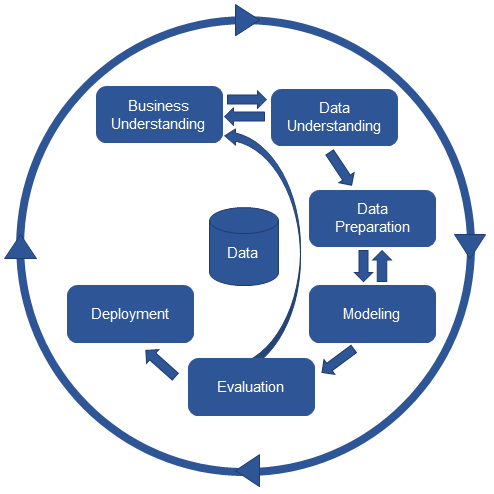
\includegraphics[width=0.8\linewidth]{Chapters/img/crisp_dm.png}
\caption{The complete CRISP-DM Approach  \cite{WEBSITE:CRISPDM}.  }
\label{fig:crisp_dm}
\end{figure}

In the following, we outline each phase briefly:
\begin{itemize}
\item Business Understanding\\
This initial phase focuses on understanding the project objectives and requirements from a
business perspective, and then converting this knowledge into a data mining problem
definition, thus a preliminary project plan designed to achieve the objectives are drown.
\item Data Understanding\\
The data understanding phase starts with an initial data collection and proceeds with activities
to get familiar with the data, to identify data quality problems, to discover first
insights into the data, or to detect interesting subsets to form hypotheses for hidden
information.
There is a close link between Business Understanding and Data Understanding. The
formulation of the data mining problem and the project plan require at least some
understanding of the available data.
\item Data Preparation\\
The data preparation phase covers all activities to construct the final dataset (data that will be
fed into the modeling tool(s)) from the initial raw data. Data preparation tasks are likely to be
performed multiple times, and not in any prescribed order. Tasks include a table, record, and attribute selection, data cleaning, construction of new attributes, and transformation of data for
modeling tools.
\item Modeling\\
In this phase, various modeling techniques are selected and applied, and their parameters are
calibrated to optimal values. Typically, there are several techniques for the same data mining
problem type. Some techniques require specific data formats.
There is a close link between Data Preparation and Modeling. Often, one realizes data
problems while modeling, or one gets ideas for constructing new data.
\item Evaluation\\
At this stage in the project, you have built one or more models that appear to have high quality,
from a data analysis perspective. Before proceeding to the final deployment of the model, it is
essential to more thoroughly evaluate the model, and review the steps executed to construct
the model, to be sure it accurately achieves the business objectives. A key objective is to
determine if there is some critical business issue that has not been sufficiently considered.
At the end of this phase, a decision on the use of the data mining results should be reached.
\item Deployment\\
The creation of the model is generally not the end of the project. Usually, the knowledge gained
will need to be organized and presented in a way that the customer can use it. Depending on
the requirements, the deployment phase can be as simple as generating a report or as complex
as implementing a repeatable data mining process. In many cases, it will be the user, not the
data analyst, who will carry out the deployment steps. In any case, it is important to
understand upfront what actions will need to be carried out to make use of
the created models.
\end{itemize}
% section crisp_dm (end)


\subsection{Data Mining Classification Algorithms}

\subsubsection{Decision Trees}
\label{subsub:decision_trees}
While in data mining, a decision tree is a predictive model that can be used to represent both classifiers and regression models. In operations research decision trees refer to a hierarchical model of decisions and their consequences\cite{Rokach2014}. The decision-maker employs decision trees to identify the strategy which will most likely reach its goal. When a decision tree is used for classification tasks, it is most commonly referred to as a classification tree. When it is used for regression tasks, it is called a regression tree \cite{Rokach2014}.
Algorithms for constructing decision trees usually work top-down, by choosing a variable at each step that best splits the set of items \cite{ApplicationsReviews}.\\
Thus, when the target variable is a discrete set of values the model is called a classification tree; In the tree structure, leaves represent class labels and branches represent features conditions corresponding to those class labels. Tree models where the target variable assumes continuous values are called regression trees.
ID3,CART and C4.5 are basically most common decision tree algorithms in data mining. They use different splitting criteria for splitting the node at each level to form a homogeneous node.
In this work, it will be used to measure the quality of a split "gini" \ref{eq:gini} for the Gini impurity (CART)\cite{DTAnalysis} and "entropy" \ref{eq:entropy} for the information gain (C4.5)\cite{DTAnalysis}.

\begin{equation}
Gini = 1 - \sum_{i=1}^{n} (P_{i})^{2}
\label{eq:gini}
\end{equation}
Where ~$P_{i}$ denotes the probability of an element being classified for a distinct class.

\begin{equation}
Entropy = \sum_{i=1}^{n} -p_{i} log_{2}(p_{i})
\label{eq:entropy}
\end{equation}
Where ~$p$ denotes the probability that it is a function of entropy.


\subsubsection{Random Forests}
\label{subsub:random_forests}
Random forests are a combination of tree predictors such that each tree depends on the values of a random vector sampled independently and with the same distribution for all trees in the forest\cite{Breiman2001}. The generalization error for forests converges a.s. To a limit as the number of trees in the forest becomes large. The generalization error of a forest of tree classifiers depends on the strength of the individual trees in the forest and the correlation between them.
A random forest is a classifier consisting of a collection of tree-structured
classifiers \(\{h(\textbf{x}, \theta \textsubscript{k} ), k = 1,...\}\) where the \( \{ \theta \textsubscript{k} \}\) are independent identically distributed
random vectors and each tree casts a unit vote for the most popular class at input \textbf{x}\cite{Breiman2001}.
The number of trees in the forest are called estimators, which the algorithm builds before taking the maximum voting or taking the averages of predictions. In general, a higher number of trees increases the performance and makes the predictions more stable, but it also slows down the computation.

\subsubsection{Neural Network}
\label{subsub:neural_network}
Neural networks are a bio-inspired mechanism of data processing that enables computers to learn technically similar to a brain and even generalize once solutions to enough problem instances are tough \cite{Kriesel2007NeuralNetworks}. An artificial neural network consists of simple processing units, the neurons, and directed, weighted connections between those neurons. A neural network is a sorted triple \((N, V, \varpi )\) with two sets N, V and a function \(\varpi\), where N is the set of neurons and V a set \(\{ (i, j) i, j \in \mathbb{N} \}\) whose elements are called connections between neuron i and neuron j. The function \( \varpi : V \rightarrow \mathbb{R}\) defines the weights, where \(\varpi(i, j)\), the weight of the connection between neuron \(i$ and neuron \(j$, is shortened to \(\varpi \textsubscript{ i,j}\) . Depending on the point of view, it is either undefined or 0 for connections that do not exist in the network \cite{Kriesel2007NeuralNetworks}. \\
In this work, we will train models with different hidden layer sizes. The solver for weight optimization used is BFGS\cite{Dai2013} and Adam\cite{adamNN} for large sizes of hidden layers.

\subsubsection{Support Vector Machine}
\label{subsub:svm}
The folklore view of SVM is that they find an optimal hyperplane as the solution to the learning problem. The simplest formulation of SVM is the linear one, where the hyperplane lies in the space of the input data \(x\). In this case, the hypothesis space is a subset of all hyperplanes of the form:
\(f(x) = w \cdotp x +b\).
In their most general formulation, SVM finds a hyperplane in a space different from that of the input data x. It is a hyperplane in a feature space induced by a kernel K (the kernel defines a dot product in that space)\cite{SVMEvgeniou}.\\
In this work, we will create models using the following kernel algorithms: Linear\cite{SVMTraining}, Polynomial\cite{SVMTraining}, and RBF\cite{SVMTraining}. 




